\documentclass[aspectratio=169]{beamer}

\usepackage{graphicx}
\usepackage{booktabs}
\usepackage{tabularx}
\usepackage{appendixnumberbeamer}
\usepackage{tikz}
\usetikzlibrary{arrows.meta,positioning}
\usepackage[scaled]{helvet}
\renewcommand{\familydefault}{\sfdefault}
\usepackage[table]{xcolor}

\definecolor{brandgreen}{HTML}{00AA5A}
\definecolor{branddark}{HTML}{333333}

\setbeamercolor{normal text}{fg=branddark,bg=white}
\setbeamercolor{background canvas}{bg=white}
\setbeamercolor{structure}{fg=brandgreen}
\setbeamercolor{title}{fg=branddark}
\setbeamercolor{frametitle}{fg=branddark}
\setbeamercolor{author in head/foot}{fg=branddark,bg=white}
\setbeamercolor{date in head/foot}{fg=branddark,bg=white}
\setbeamertemplate{navigation symbols}{}

% Frametitle with thin brand line.
\setbeamertemplate{frametitle}{%
  \vspace*{0.2em}%
  \usebeamerfont{frametitle}\insertframetitle\par
  {\color{brandgreen}\rule{\textwidth}{0.6pt}}\vspace{-0.25em}%
}

% Footline with institute left and slide count right.
\setbeamertemplate{footline}{%
  \leavevmode\hbox{%
    \begin{beamercolorbox}[wd=.80\paperwidth,ht=2.5ex,dp=1ex,left]{author in head/foot}%
      \hspace*{1em}\usebeamerfont{author in head/foot}\insertshortinstitute
    \end{beamercolorbox}%
    \begin{beamercolorbox}[wd=.20\paperwidth,ht=2.5ex,dp=1ex,right]{date in head/foot}%
      \usebeamerfont{date in head/foot}\insertframenumber{} / \inserttotalframenumber\hspace*{1em}
    \end{beamercolorbox}%
  }\vskip0pt
  \begingroup\color{brandgreen}\rule{\paperwidth}{0.8pt}\endgroup
}

% Keep footline visible on [plain] frames.
\makeatletter
\def\beamer@frametemplate@plain{%
  \def\beamer@entrycode{\vspace*{-\headheight}}%
  \def\beamer@exitcode{\vspace*{-\footheight}}%
}
\makeatother

% Section divider slides with optional mini-TOC.
\newif\ifsectionoverview
\sectionoverviewtrue
\AtBeginSection[]{
  \begin{frame}[plain]
    \centering
    {\Huge\bfseries \insertsection\par}
    \ifsectionoverview
      \vspace{0.8em}
      \tableofcontents[currentsection]
    \fi
  \end{frame}
}

% Metadata (edit for your project).
\newcommand{\thesistitle}{Your Thesis Title}
\newcommand{\authorname}{Your Name}
\newcommand{\supervisor}{Supervisor Name}
\newcommand{\instituteabbr}{Example University}

\title{\thesistitle}
\subtitle{Supervisor: \supervisor}
\author[\authorname]{\authorname}
\institute{\instituteabbr}
\date{\today}

\begin{document}

% Title frame with top-right logo if available.
{
\setbeamertemplate{footline}{}
\begin{frame}[plain,noframenumbering]
  \begin{tikzpicture}[remember picture,overlay]
    \IfFileExists{assets/logo.png}{%
      \node[anchor=north east,xshift=-0.6cm,yshift=-0.4cm] at (current page.north east)
        {\includegraphics[height=1.2cm]{assets/logo.png}};
    }{}
  \end{tikzpicture}
  \titlepage
\end{frame}
}

\begin{frame}[plain]
  \frametitle{Outline}
  \tableofcontents
\end{frame}

\section{Motivation}
\begin{frame}[plain]
  \frametitle{Research Context}
  \begin{columns}[T,totalwidth=\textwidth]
    \begin{column}{0.58\textwidth}
      \begin{itemize}
        \item Briefly explain the problem domain.
        \item State the gap in current methods or tooling.
        \item Define the concrete thesis objective.
      \end{itemize}
    \end{column}
    \begin{column}{0.38\textwidth}
      \fbox{\parbox[c][0.48\textheight][c]{\linewidth}{\centering
        Optional intro figure\\
        \texttt{assets/intro-figure.pdf}
      }}
    \end{column}
  \end{columns}
\end{frame}

\section{Methods}
\begin{frame}[plain]
  \frametitle{Workflow at a Glance}
  \centering
  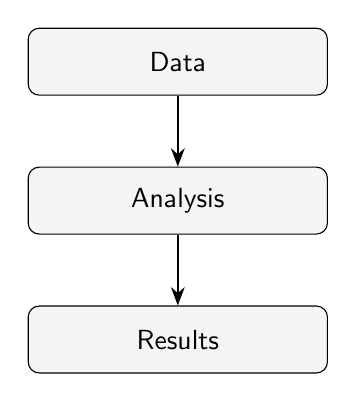
\begin{tikzpicture}[
    node distance=0.9cm,
    box/.style={draw, rounded corners, fill=black!4, minimum width=3.8cm, minimum height=0.85cm, align=center},
    arrow/.style={->, thick, >=Stealth}
  ]
    \node[box] (input) {Data};
    \node[box, below=of input] (analysis) {Analysis};
    \node[box, below=of analysis] (output) {Results};

    \draw[arrow] (input) -- (analysis);
    \draw[arrow] (analysis) -- (output);
  \end{tikzpicture}
\end{frame}

\begin{frame}[plain]
  \frametitle{Study Plan (Example)}
  \small
  \begin{tabularx}{\textwidth}{l X c c}
    \toprule
    ID & Task & Priority & Status \\
    \midrule
    T1 & Baseline setup and metrics definition & High & Done \\
    T2 & Method comparison and sensitivity checks & High & In progress \\
    T3 & Robustness and ablation experiments & Medium & Planned \\
    \bottomrule
  \end{tabularx}
\end{frame}

\section{Results}
\begin{frame}[plain]
  \frametitle{Main Result Placeholder}
  \begin{columns}[T,totalwidth=\textwidth]
    \begin{column}{0.62\textwidth}
      \fbox{\parbox[c][0.52\textheight][c]{\linewidth}{\centering
        Insert main result figure\\
        \texttt{figures/main-result.pdf}
      }}
    \end{column}
    \begin{column}{0.35\textwidth}
      \begin{itemize}
        \item Key finding 1
        \item Key finding 2
        \item Quantitative takeaway
      \end{itemize}
    \end{column}
  \end{columns}
\end{frame}

\section{Conclusion}
\begin{frame}[plain]
  \frametitle{Takeaways}
  \begin{itemize}
    \item Summarize the core contribution in one sentence.
    \item Mention practical implications or limitations.
    \item List clear next steps.
  \end{itemize}
\end{frame}

\begin{frame}[plain,noframenumbering]
  \centering
  {\LARGE Thank You}\\[0.6em]
  Questions?
\end{frame}

\appendix
\section{Backup}
\begin{frame}[plain]
  \centering
  {\Large Backup Slides}
\end{frame}

\end{document}
